\chapter{Dataset}%    \chapter{}  = level 1, top level


	\section{Introduction to container dataset}
		The dataset has records regarding container terminal operations. More over 1.5 million observations and 35
		variables provide a detailed details container movements, including imports, exports, and container features.


	\section{Data Features Overview}

		The dataset encompasses a comprehensive set of features that characterize container operations at the port.
		These features can be categorized into five main groups. As shown in Table \ref{tab:container_chars}
		, categorical features include container physical characteristics such as nominal length (20, 40,
		45, or 10 feet) and location types. The operational categories, detailed in Table \ref{tab:category_features}
		, include import (IMPRT), export (EXPRT), storage (STRGE), transshipment (TRSHP), and through cargo (
		THRGH). Table \ref{tab:move_kind}
		outlines the movement types captured through various categories like delivery (DLVR), loading (LOAD),
		yard moves (YARD), and others, while freight types are classified in Table \ref{tab:freight_kind}
		as either empty (MTY) or full container load (FCL).

		\begin{table}[H]
			\centering
			\begin{tabular}{p{0.2\textwidth}p{0.7\textwidth}}
				\hline
				\textbf{Column Name} & \textbf{Description}
				\\
				\hline
				nominal\_length & Container size that could be 20, 40, 45, and 10
				\\
				\hline
				arrive\_pos\_loctype & Type of location arrival
				\\
				\hline
				last\_pos\_loctype & Last position's type where the container was fetched from, related to fm\_pos
				\_locid \\
				\hline
			\end{tabular}
			\caption{Container Characteristics Features}
			\label{tab:container_chars}
		\end{table}

		\begin{table}[H]
			\centering
			\begin{tabular}{p{0.15\textwidth}p{0.7\textwidth}}
				\hline
				\textbf{Category} & \textbf{Description}                                                  \\
				\hline
				IMPRT                 & Import                                                                \\
				\hline
				EXPRT                 & Export                                                                \\
				\hline
				STRGE                 & Storage                                                               \\
				\hline
				TRSHP                 & When a box comes off a vessel and goes on another vessel              \\
				\hline
				THRGH                 & When a box leaves on the same vessel it came on, it just went through \\
				\hline
			\end{tabular}
			\caption{Container Category Features}
			\label{tab:category_features}
		\end{table}

		\begin{table}[H]
			\centering
			\begin{tabular}{p{0.15\textwidth}p{0.7\textwidth}}
				\hline
				\textbf{Category} & \textbf{Description} \\
				\hline
				DLVR                  & Delivery             \\
				\hline
				LOAD                  & Load                 \\
				\hline
				YARD                  & Yard Move            \\
				\hline
				SHFT                  & Yard Shift           \\
				\hline
				RECV                  & Receival             \\
				\hline
				RLOD                  & Rail load            \\
				\hline
				OTHR                  & Other                \\
				\hline
				RDSC                  & Rail Discharge       \\
				\hline
				DSCH                  & Discharge            \\
				\hline
				SHOB                  & Shift O.B            \\
				\hline
			\end{tabular}
			\caption{Move Kind Features}
			\label{tab:move_kind}
		\end{table}

		\begin{table}[H]
			\centering
			\begin{tabular}{p{0.15\textwidth}p{0.7\textwidth}}
				\hline
				\textbf{Category} & \textbf{Description} \\
				\hline
				MTY                   & Empty                \\
				\hline
				FCL                   & Full Container Load  \\
				\hline
			\end{tabular}
			\caption{Freight Kind Features}
			\label{tab:freight_kind}
		\end{table}

		Binary features, presented in Table \ref{tab:binary_features}
		, track specific operational requirements such as power needs for temperature-sensitive cargo and twin
		operation capabilities (fetch, carry, and put).

		\begin{table}[H]
			\centering
			\begin{tabular}{p{0.2\textwidth}p{0.7\textwidth}}
				\hline
				\textbf{Column Name} & \textbf{Description}
				\\
				\hline
				requires\_
				power & Container designed to be transported as temperature sensitive cargo with precisely
				controlled temperatures \\
				\hline
				twin\_fetch & Pairs of containers that were able be twin fetched
				\\
				\hline
				twin\_carry & Pairs of containers that can able be twin carried
				\\
				\hline
				twin\_put & Time when the whole chain of events related to a container\_visit\_
				gkey is completed \\
				\hline
			\end{tabular}
			\caption{Binary Features}
			\label{tab:binary_features}
		\end{table}

		Temporal information is captured through datetime features, listed in Table \ref{tab:datetime_features}
		, that record crucial timestamps including port arrival (time\_in), departure (time\_out), and various
		handling operations (t\_put, t\_dispatch, t\_fetch, t\_discharge).
		\begin{table}[H]
			\centering
			\begin{tabular}{p{0.2\textwidth}p{0.7\textwidth}}
				\hline
				\textbf{Column Name} & \textbf{Description}
				\\
				\hline
				t\_put & Time completed
				\\
				\hline
				t\_dispatch & Time when a container is dispatched somewhere like on a vessel or truck
				\\
				\hline
				t\_carry\_dispatch & Requires verification
				\\
				\hline
				t\_fetch & Datetime when the container was fetched
				\\
				\hline
				t\_discharge & Datetime when container is left in position after being fetched
				\\
				\hline
				time\_
				in & Datetime of port arrival (for transships: can indicate category change from
				storage
				to export) \\
				\hline
				time\_out & Time when the container leaves the port
				\\
				\hline
			\end{tabular}
			\caption{Datetime Features}
			\label{tab:datetime_features}
		\end{table}

		Table \ref{tab:numerical_features}
		outlines numerical features that provide quantitative data about container handling, including rehandle
		counts, weight measurements (goods\_an\d_ctr\_wt\_kg), and movement distances (dist\_start, dist\_carry).
		\begin{table}[H]
			\centering
			\begin{tabular}{p{0.2\textwidth}p{0.7\textwidth}}
				\hline
				\textbf{Column Name} & \textbf{Description}
				\\
				\hline
				rehandle\_count & Number of times a container was rehandled
				\\
				\hline
				goods\_and\_ctr\_wt\_kg & Total weight of goods and container
				\\
				\hline
				dist\_start & Distance where container started to be moved
				\\
				\hline
				dist\_
				carry & Distance container was carried during move (correlated to starting distance) \\
				\hline
			\end{tabular}
			\caption{Numerical Features}
			\label{tab:numerical_features}
		\end{table}

		Finally, identifier features, detailed in Table \ref{tab:identifier_features}
		, maintain traceability through unique keys for moves (mve\_gkey), locations (fm\_pos\_locid,
		to\_pos\_locid)
		, containers (inv\_unit\_id), and operators (bizunit\_id).

		\begin{table}[H]
			\centering
			\begin{tabular}{p{0.2\textwidth}p{0.7\textwidth}}
				\hline
				\textbf{Column Name} & \textbf{Description}                                    \\
				\hline
				mve\_gkey                & Unique identifier for each move                         \\
				\hline
				fm\_pos\_locid           & FROM Position location id associated with fm\_pos\_name \\
				\hline
				fm\_pos\_name            & Name of the location associated with fm\_pos\_locid     \\
				\hline
				to\_pos\_locid           & TO Position location associated with to\_pos\_name      \\
				\hline
				to\_pos\_name            & Name of the location associated with to\_pos\_locid     \\
				\hline
				inv\_unit\_id            & Container ID (persistent across port visits)            \\
				\hline
				bizunit\_id              & Line operator's ID                                      \\
				\hline
			\end{tabular}
			\caption{Identifier Features}
			\label{tab:identifier_features}
		\end{table}


	\section{Data Preprocessing}

		\subsection{Data Augmentation}

			From existing features (table~\ref{tab:datetime_features}
			),new ones like the month, day, week of the month, day of the week, and even the time each container
			arrived were created based on the dates. Also, the number of days for each container, related to dwell
			time, was calculated using the dates in and out, creating the feature: "Days in the port category," a range
			of days.

		\subsection{Data Cleaning}

			The dataset was almost complete for the approach. However, some formats had to be set properly, from
			strings to dates. It had some columns with flags (like requires\_
			power) that had missing values. For these, an imputation with 0 was done.

		\subsection{Data Reduction}
			Our final dataset was reduced into 480,625 rows, each representing a unique container stay with ten chosen
			features split into two main chunks:

			\begin{itemize}
				\item 376,557 rows from 2023 for training and initial testing
				\item 104,068 rows from 2024 kept separate as our unseen data for final testing
			\end{itemize}
			The year 2024 was set up to test the model's performance on truly new data – the ultimate test of its
			predictive power.
			\\
			\\
			Many columns containing IDs, session user information, dates, and flags outside the goal of predicting
			dwell time were removed.
			\\
			\\
			After selecting the most important columns, the ones included were container's physical characteristics (
			nominal length), operational requirements (requires power status), and cargo attributes (freight kind and
			category). The temporal aspects were captured through multiple granularities: time of day (hour), day of
			week, month, business day status, week of year, and week of month.


	\section{Data analysis}

		\subsection{Initial Exploratory Approach}
			The research began with an open-ended mandate from the Ports of Auckland to analyze their operational data
			to look for potential yard optimization insights. Rather than starting with a predefined hypothesis, this
			project follows an exploratory data science approach to discover patterns and opportunities from the
			provided data. The database structure was initially understood by examining column types and their values.
			Each finding pattern was evaluated with the stakeholders from Ports of Auckland.

		\subsection{Tool Selection: R}
			R was selected for the initial data exploration because of its robust statistical analysis and
			visualization tools. Packages such as ggplot2 enabled detailed visualizations, and data packages allowed
			efficient handling of large datasets. RStudio\’s interactive environment provided quick visual feedback,
			making it easy to try different approaches rapidly. R\’s built-in statistical functions and intuitive data
			manipulation also made it ideal for exploratory work in this phase.
			\\
			\\
			R provided several clear benefits compared to Python, which was also a potential choice for data
			exploration. Its syntax allows data manipulation to be faster and easier. Also, its high-quality default
			plotting aesthetics minimized the need for extensive customization, allowing advanced customization when
			needed.
			\\
			\\
			R\’s built-in solid statistical analysis tools delivered immediate insights without extra library
			installations, and its efficient memory management was essential for effectively handling the sizeable
			operational dataset.
			\\
			\\
			This data exploration is provided in \cite{githubrepo}.

		\subsection{Iterative Development Process}
			The methodology for this project follows an iterative approach that involves an in-depth data exploration
			using R, which exposed potential optimization areas. The insights generated in this phase were part of
			follow-up discussions with Ports of Auckland stakeholders to ensure they were aligned with real operational
			needs.

		\subsection{Data Exploration}

			\begin{figure}[ht]
				\centering
				\begin{minipage}{0.5\textwidth}
					\centering
					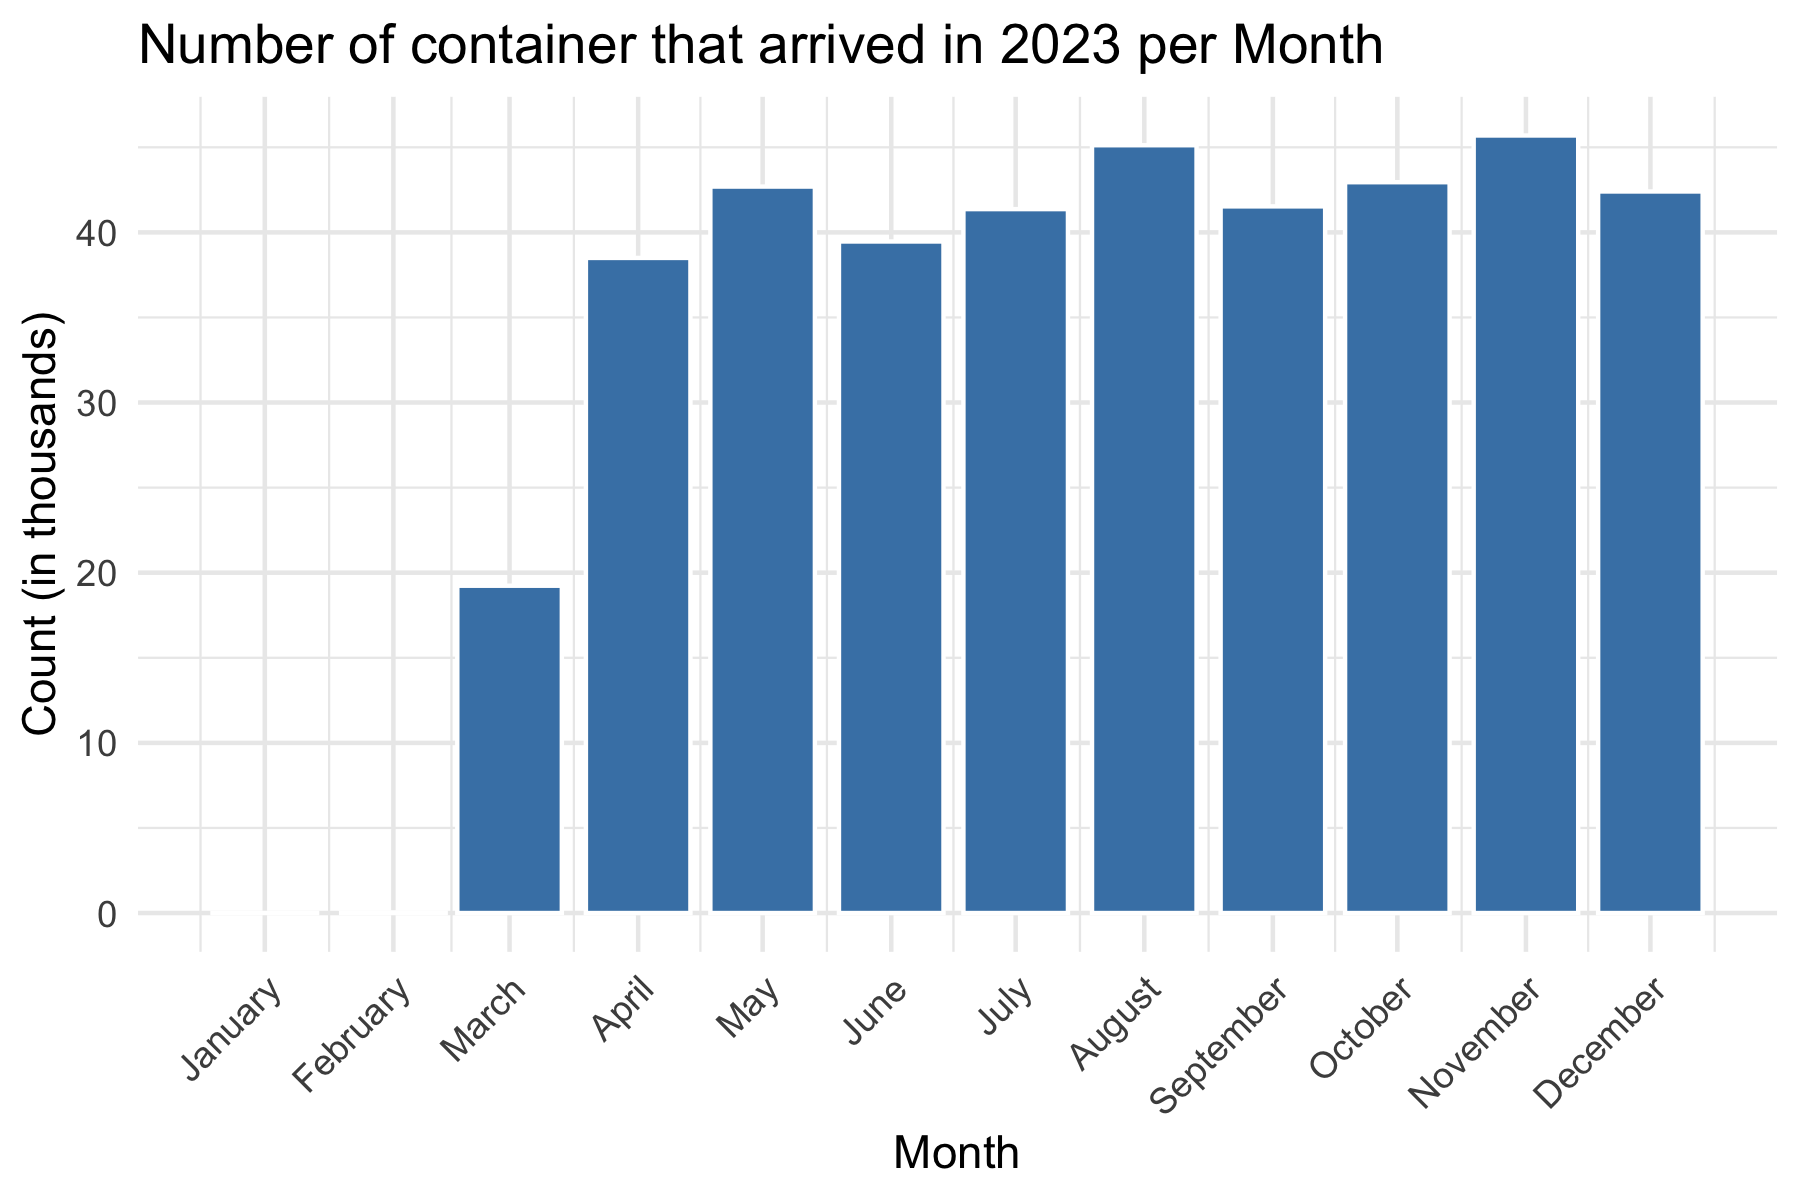
\includegraphics[width=\textwidth]{images/du_zero_one}
					\caption{Container arrivals at a port 2023}
					\label{fig:du_containers_arrivals_2023}
				\end{minipage}%
				\hfill
				\begin{minipage}{0.5\textwidth}
					\centering
					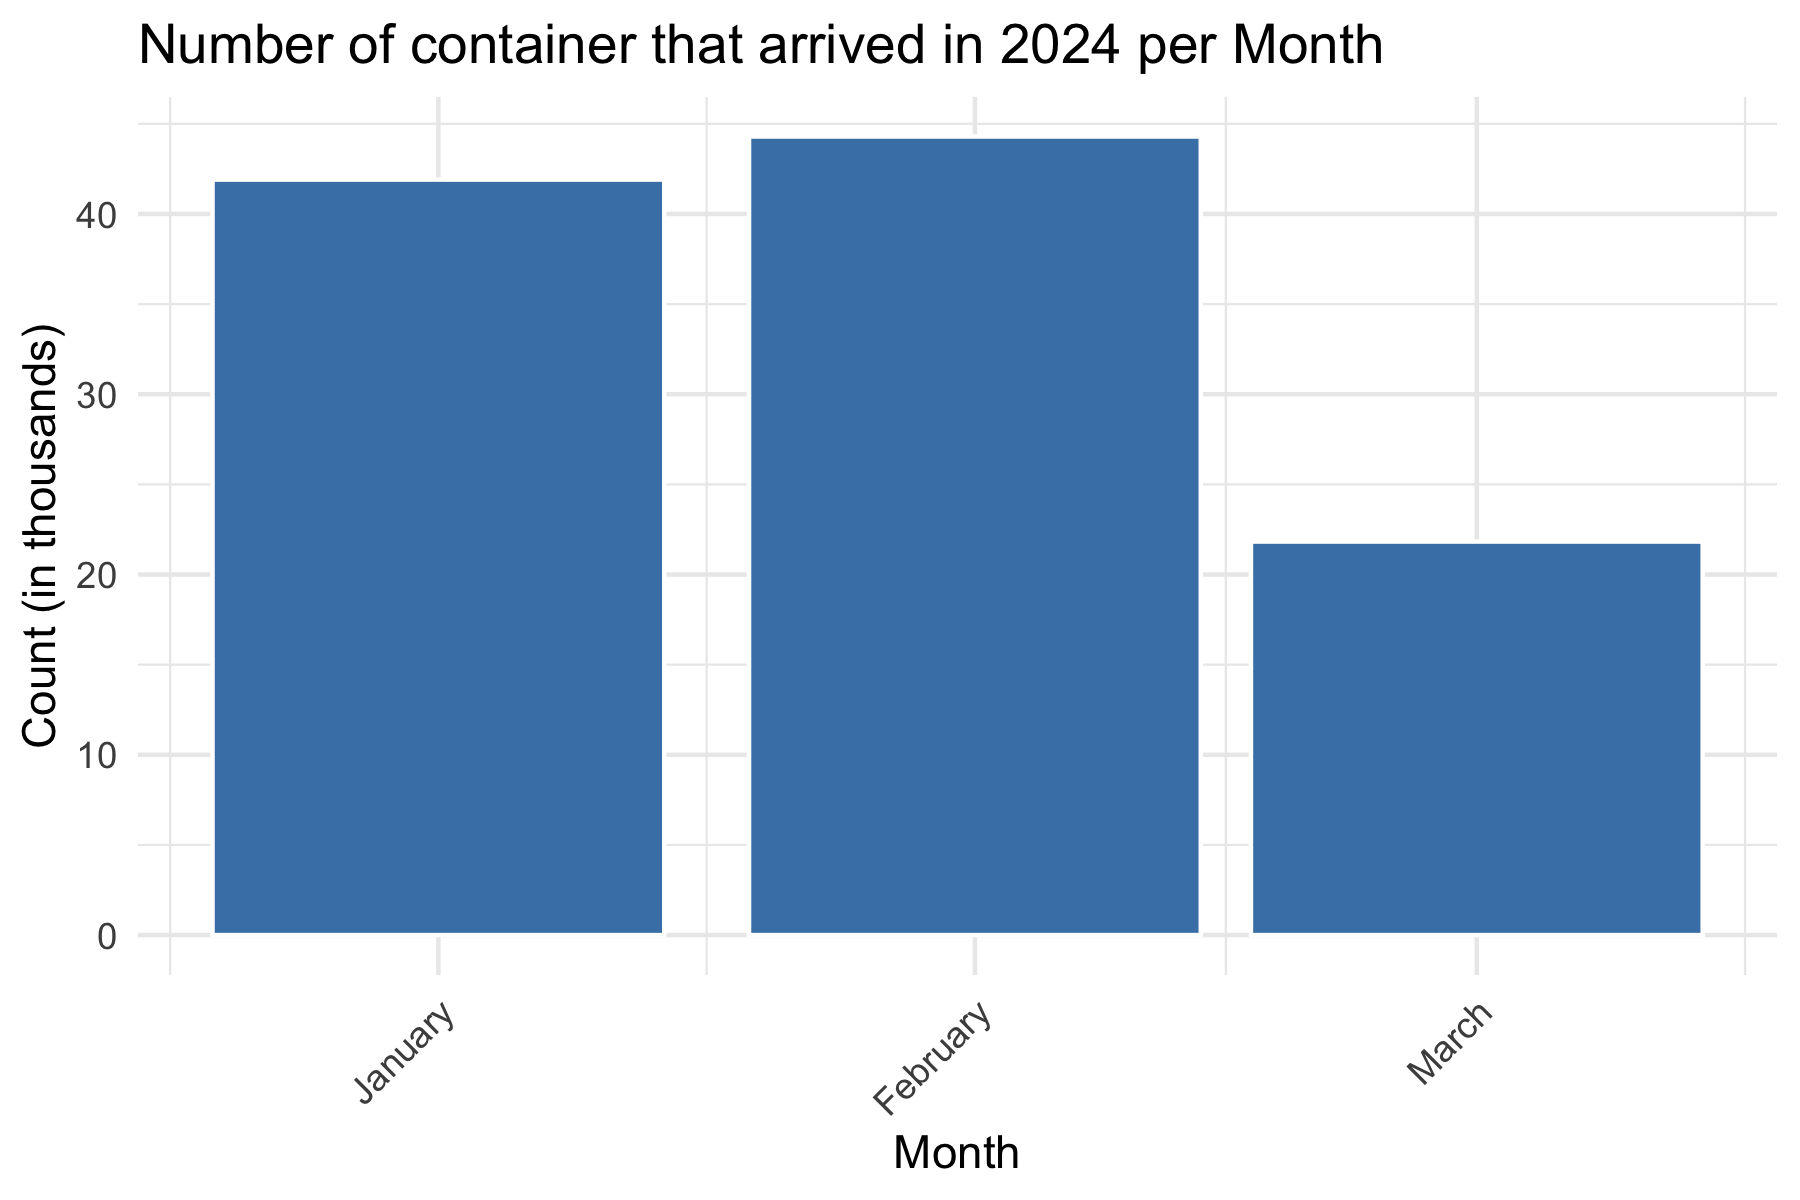
\includegraphics[width=\textwidth]{images/du_zero_two}
					\caption{Container arrivals at a port 2024}
					\label{fig:du_containers_arrivals_2024}
				\end{minipage}
			\end{figure}

			Figure~\ref{fig:du_containers_arrivals_2023}
			illustrates the monthly container arrivals at a port, measured in thousands of units, spanning
			from January 2023 to March 2024, with the 2024 cycle needing to be completed as it only covers the
			first quarter. For the year 2023, there is no available data for January and February. It includes
			half the month of March with approximately 19,000 containers.
			\\
			\\
			For April, the amount of containers reached about 38,000 containers. Throughout the remainder of
			2023, the port maintained relatively stable activity levels from May through December, with monthly
			container arrivals fluctuating between 39,000 and 45,000 units. A peak activity was observed in September,
			with approximately 45,000 containers concluding in December, with approximately 42,000 container arrivals.
			\\
			\\
			The available data for 2024 (Figure~\ref{fig:du_containers_arrivals_2024}), which only spans the first
			quarter, shows that January began with approximately 42,000 container arrivals, followed by a slight
			increase to about 45,000 containers in February. However, March contains just the first two weeks of the
			month with approximately 22,000 containers.
			\\
			\\
			\begin{figure}[ht]
				\centering
				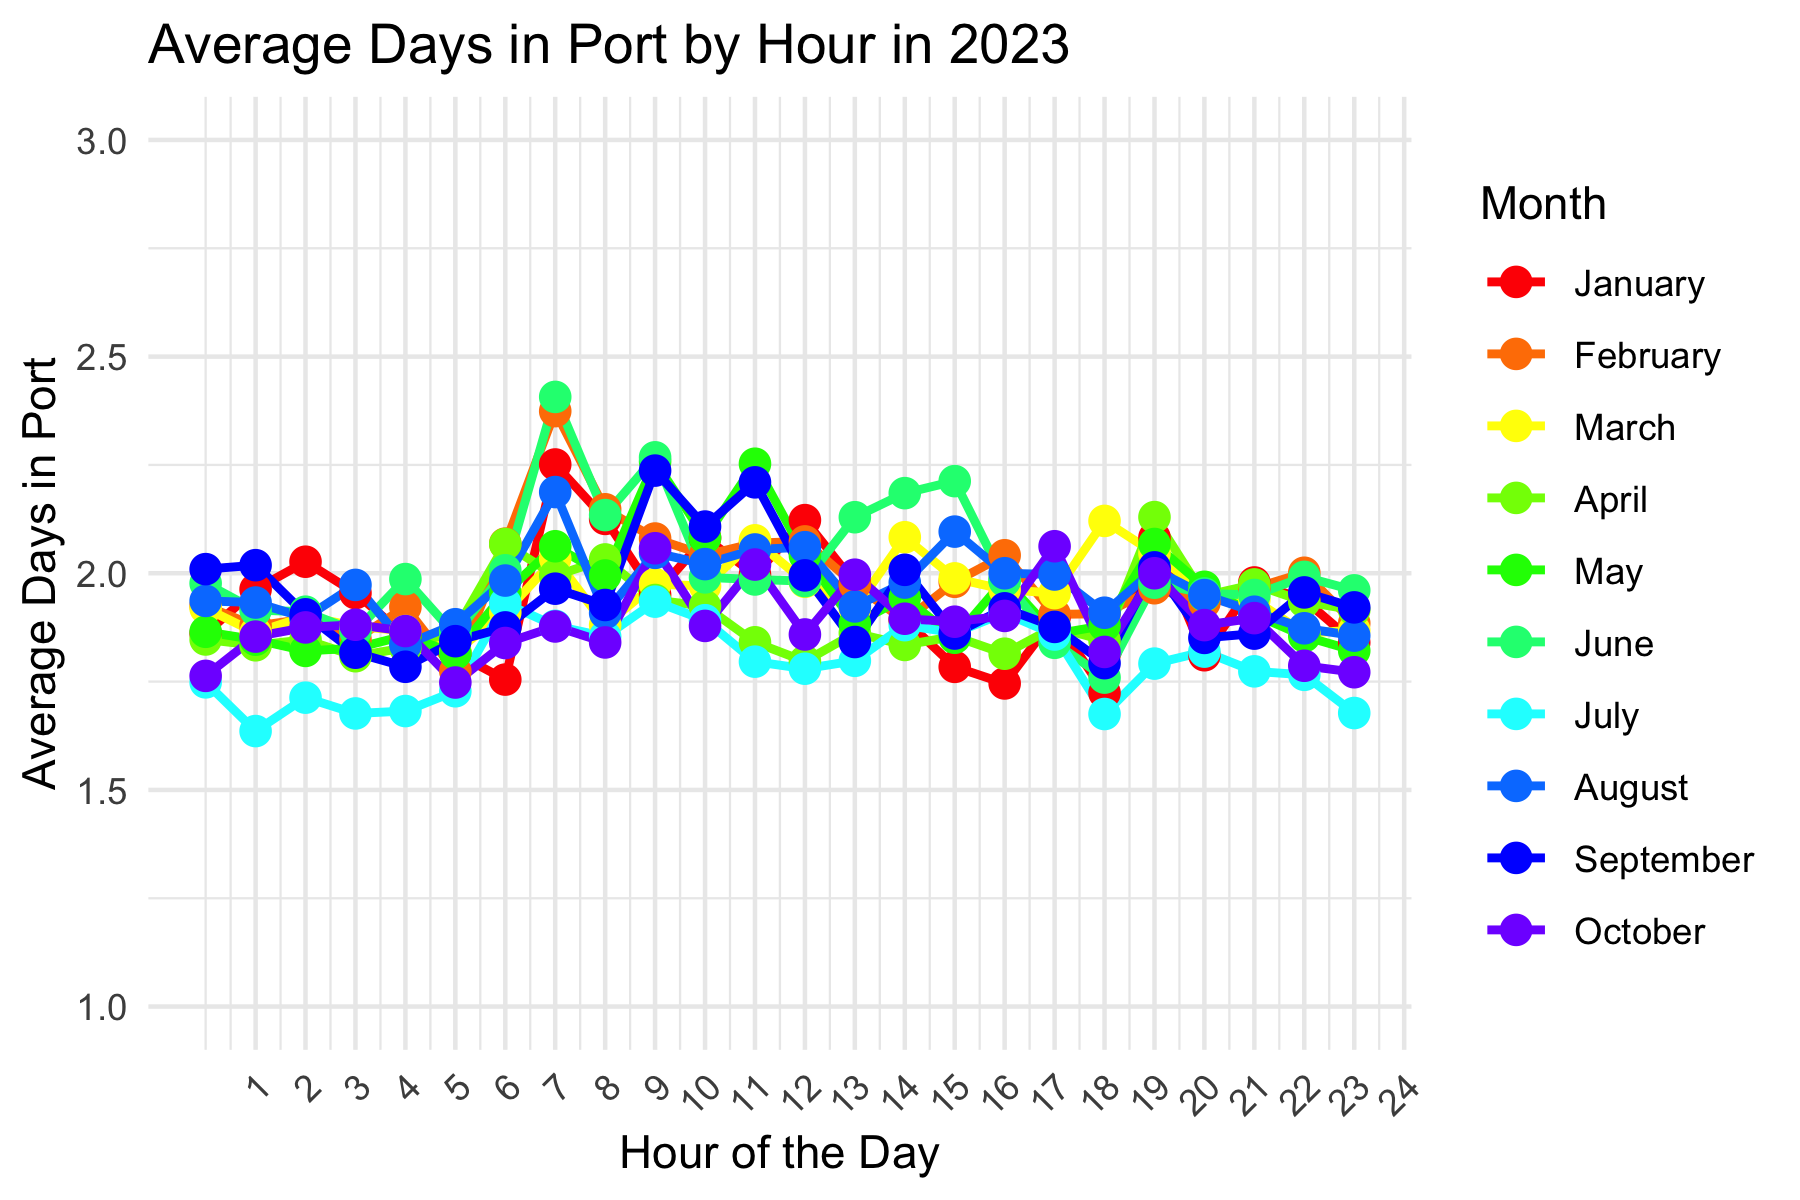
\includegraphics[width=0.8\textwidth]{images/du_seven}
				\caption{Average days in port by arrival hours per month}
				\label{fig:hourly_arrivals}
			\end{figure}
			Figure \ref{fig:hourly_arrivals} shows, in an hourly analysis of container and their dwell
			times throughout 2023 shows patterns that could be valuable for predictive modeling. The most notable
			feature is a consistent peak in dwell times during the morning (7:00-8:00 AM), where containers typically
			stay 2.2-2.4 days. This morning peak is particularly pronounced in June, which shows the highest dwell
			times during these hours. There is a cycle that starts with relatively stable dwell times of 1.8-2.0 days
			during early morning hours (1-5 AM), followed by the sharp morning peak (6-9 AM), then maintaining slightly
			elevated but more stable times during midday (10-15), before gradually declining through the afternoon and
			evening hours (16-24). These seasonal variations are evident, with summer months (June-August) having more
			volatility in dwell times, while July consistently shows lower overall dwell times than other months.
			Winter months (January-February) exhibit more consistent patterns with less variation. These interactions
			between arrival hour and month seem to be a possible factor in determining dwell times, as evidenced by
			the varying patterns across different months at specific hours. This suggests that both the hour of
			arrival and the month and their interaction term should be considered features for the predictive model.
			\\
			\\
			\begin{figure}[ht]
				\centering
				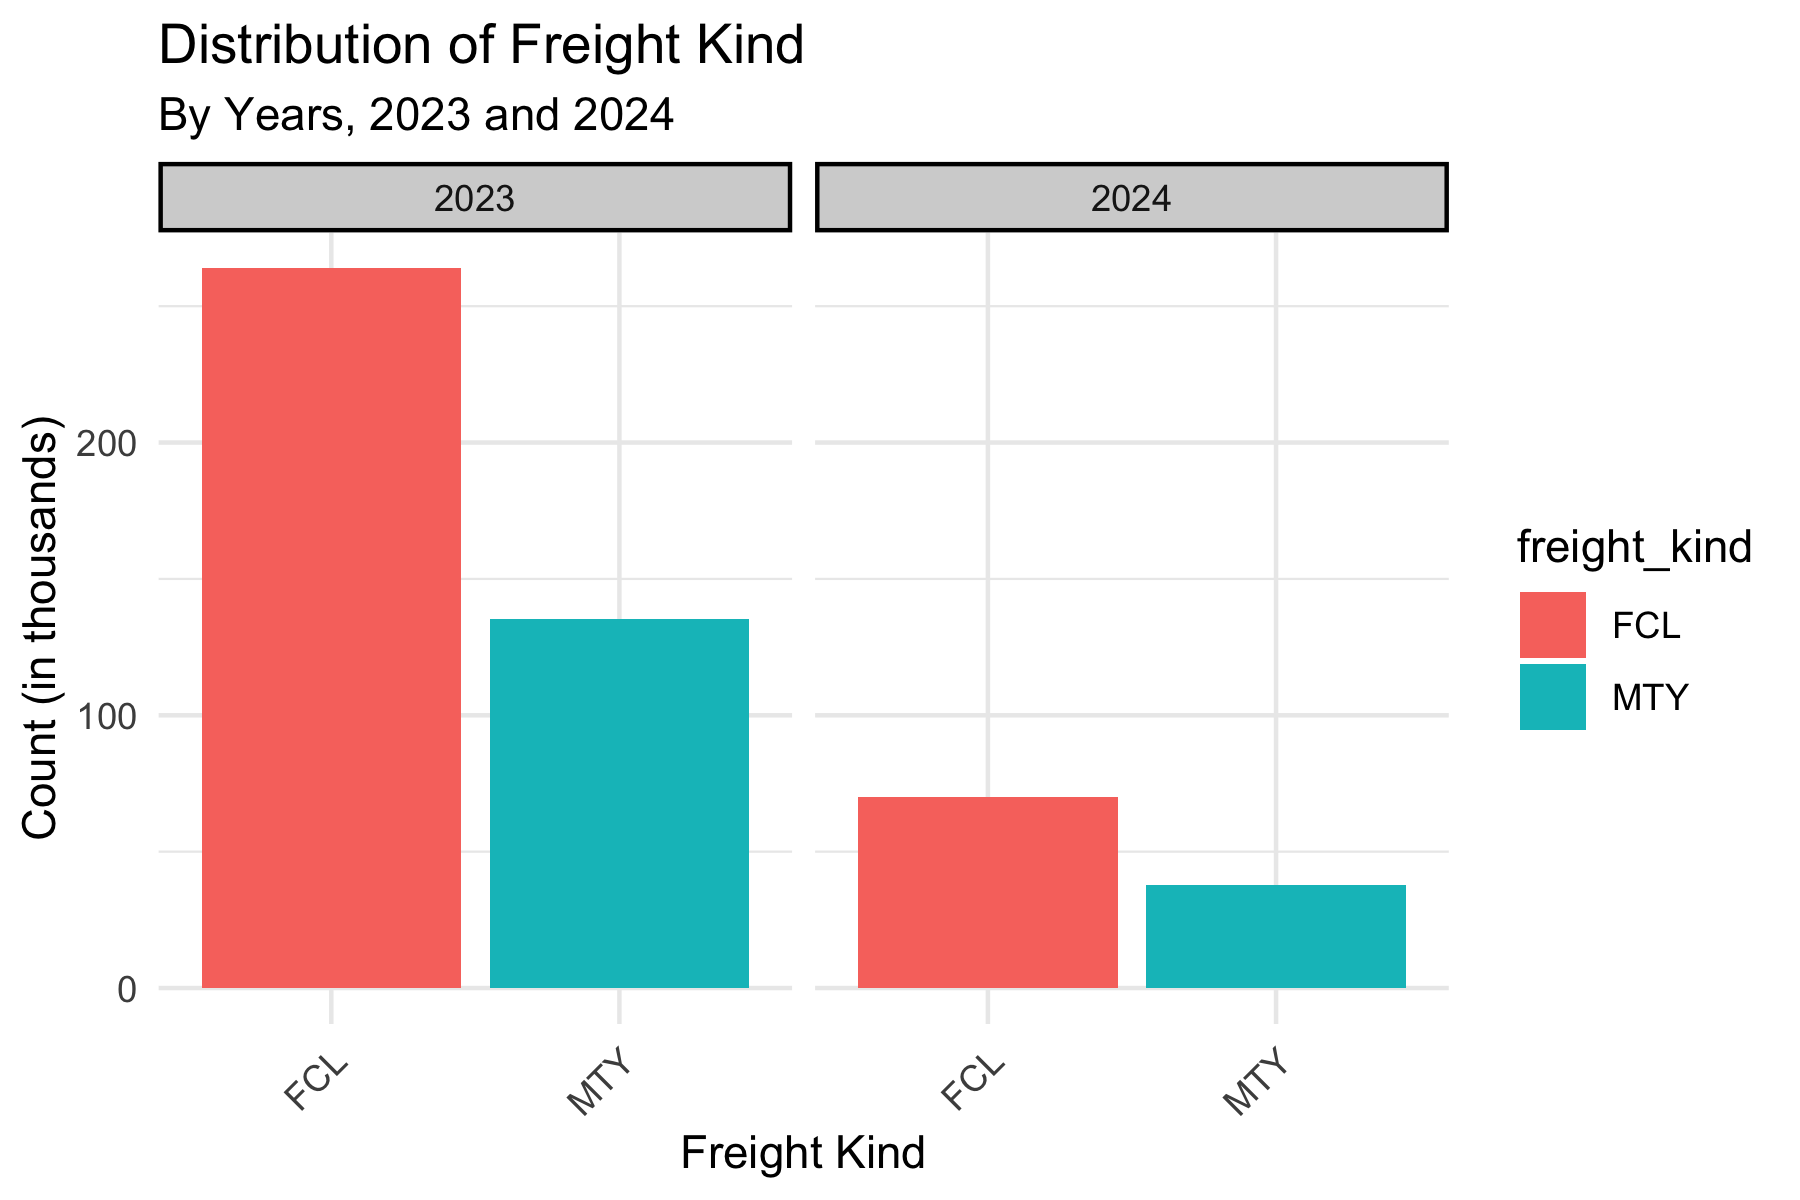
\includegraphics[width=0.5\textwidth]{images/du_four}
				\caption{Distribution of container by Freight Kind}
				\label{fig:freigh_kind_distribution}
			\end{figure}

			\begin{figure}[ht]
				\centering
				\begin{minipage}{0.5\textwidth}
					\centering
					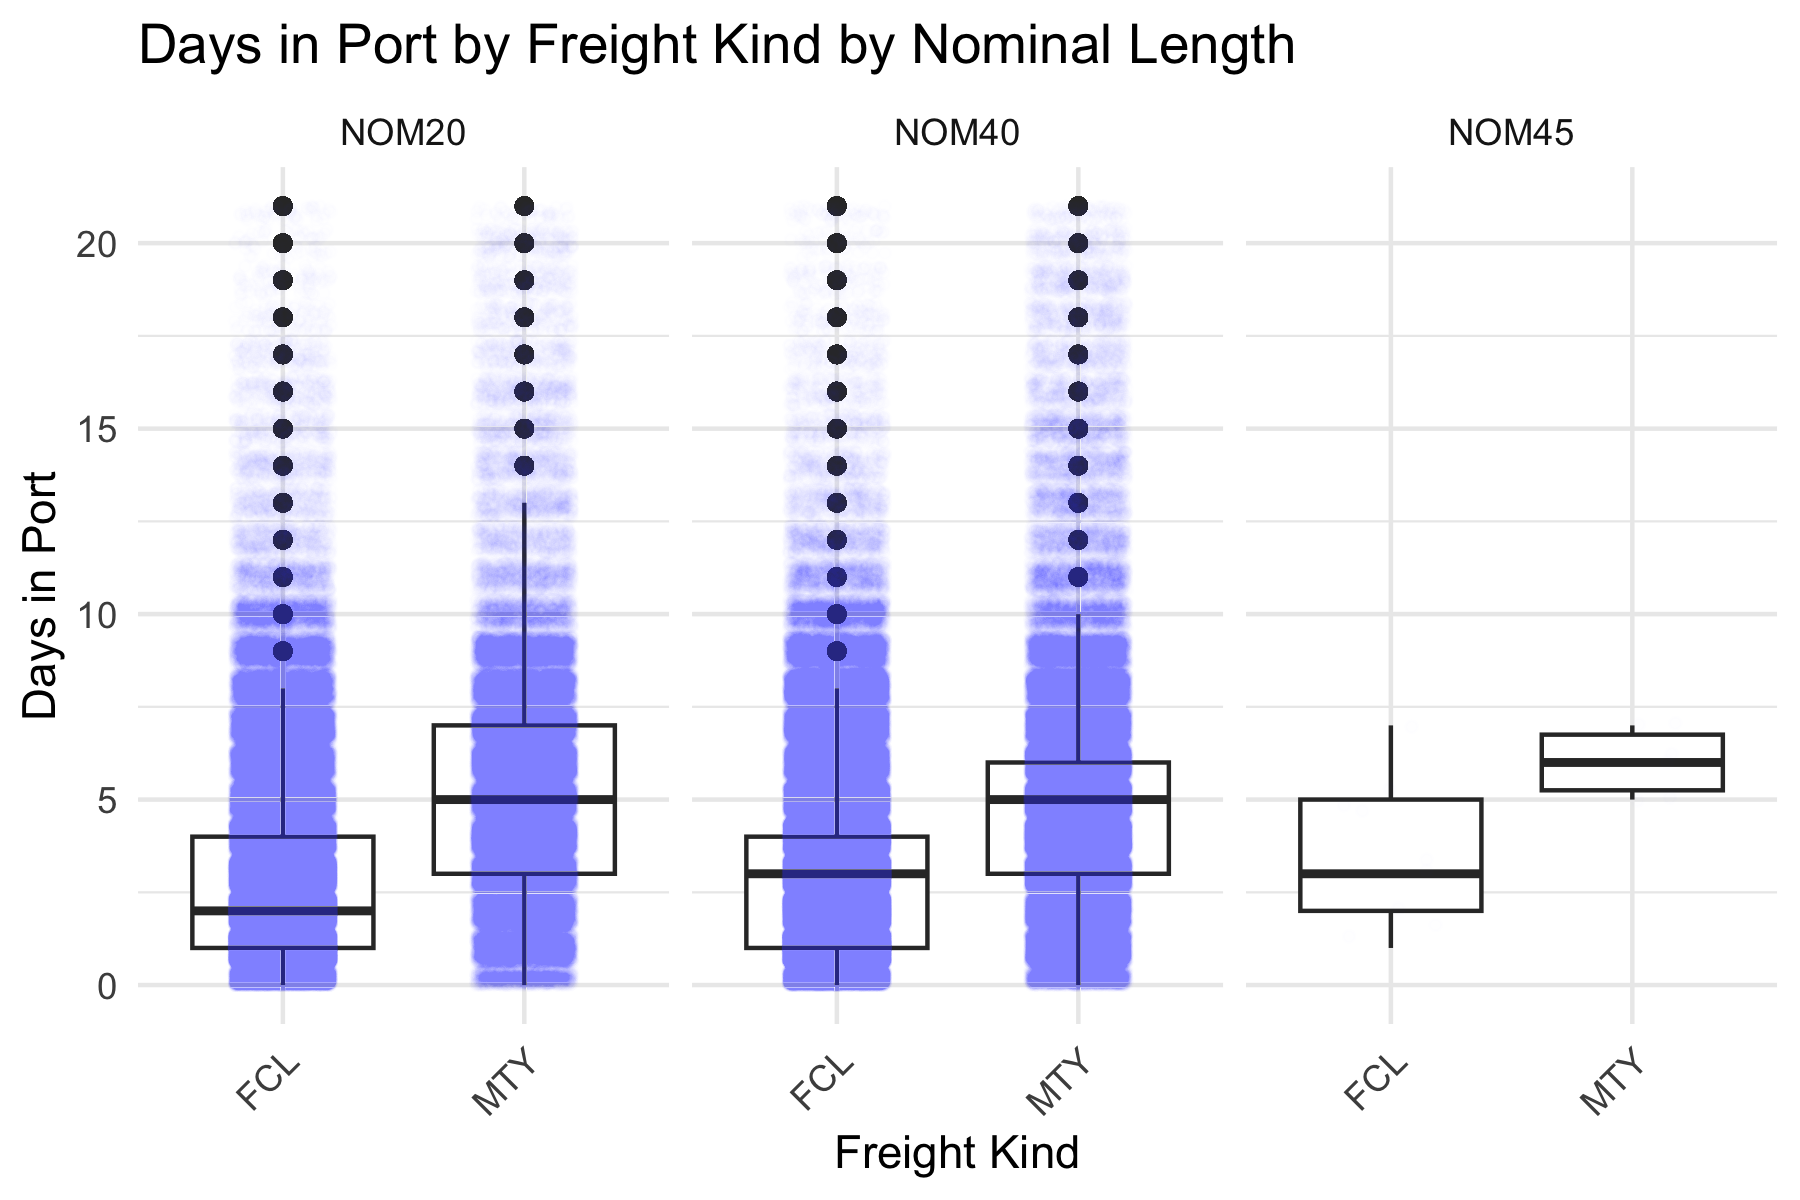
\includegraphics[width=\textwidth]{images/du_three}
					\caption{Freight kind vs size}
					\label{fig:freigh_kind_and_nominal_length}
				\end{minipage}%
				\hfill
				\begin{minipage}{0.5\textwidth}
					\centering
					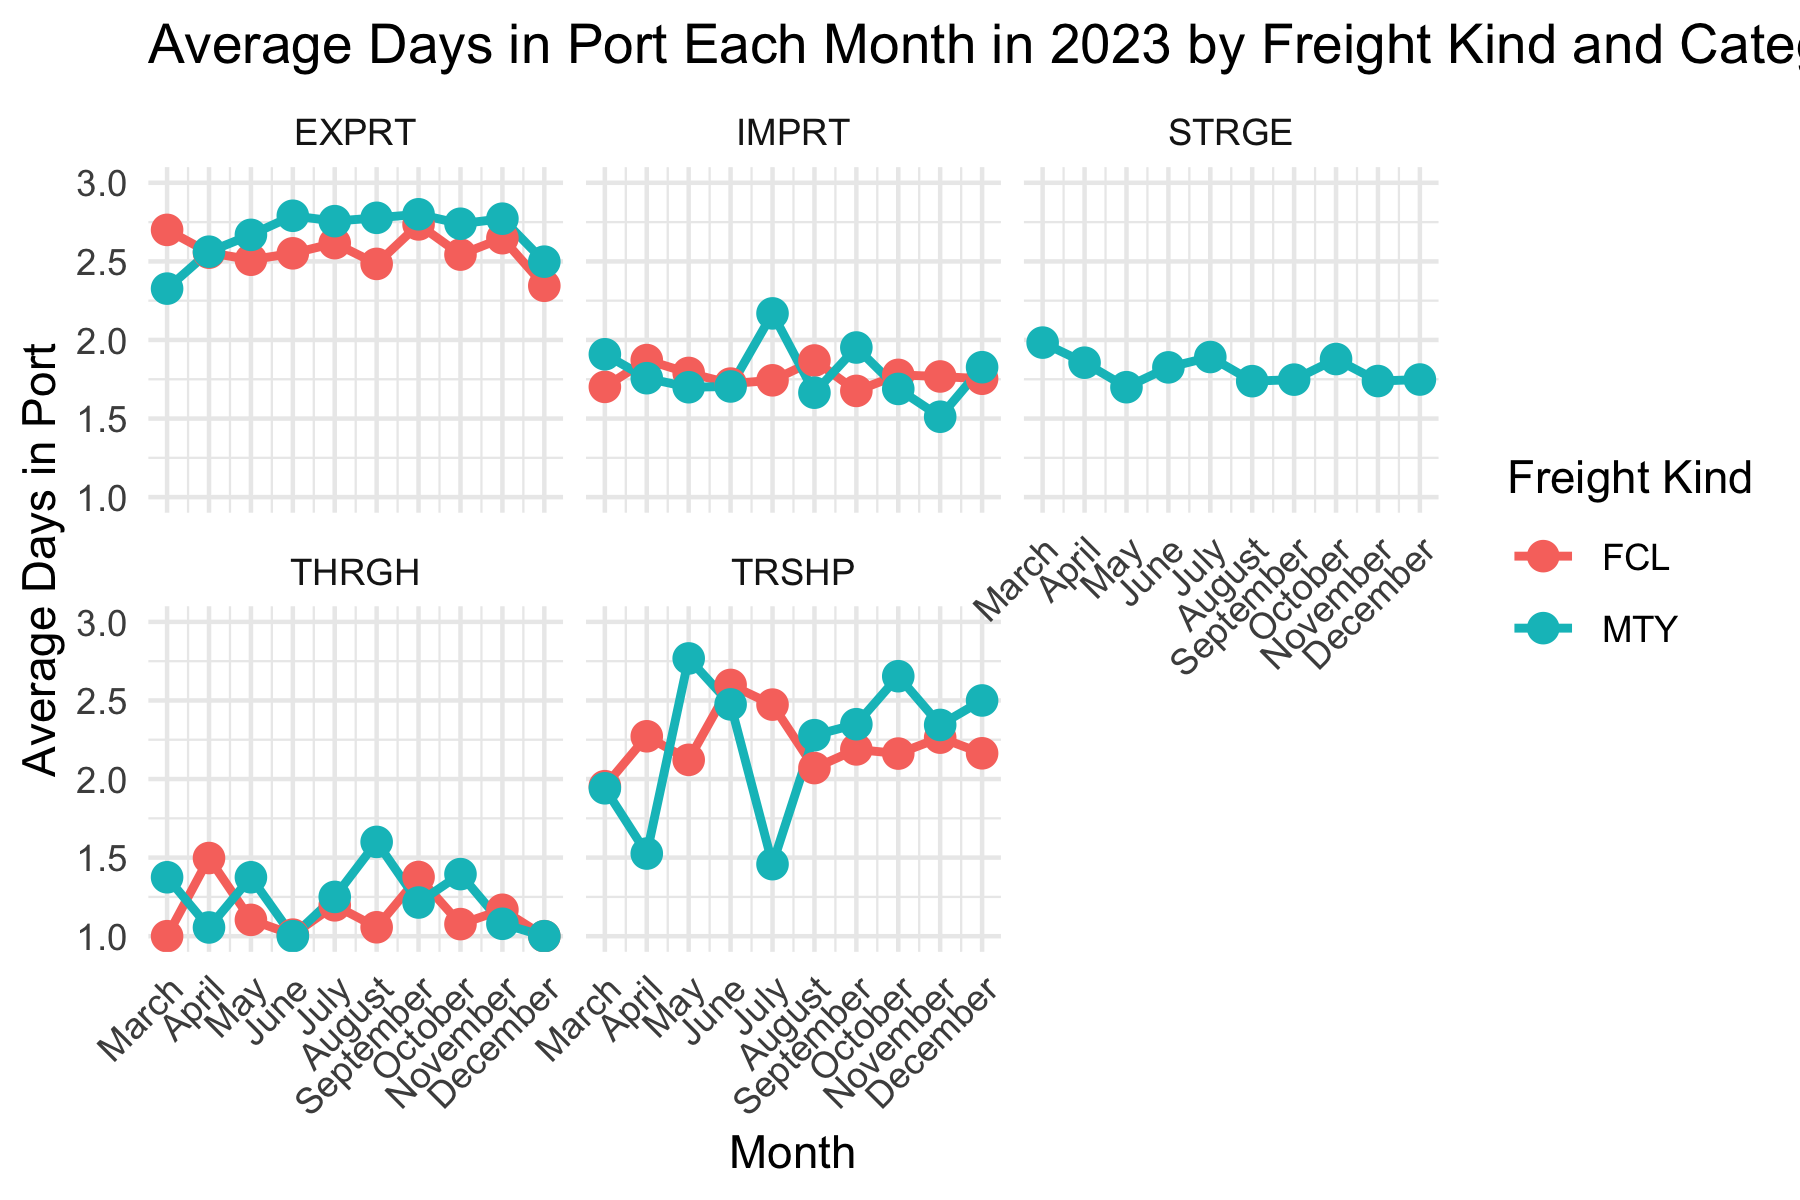
\includegraphics[width=\textwidth]{images/du_two}
					\caption{Month vs freight kind}
					\label{fig:category_freiht_kind_and_month}
				\end{minipage}
			\end{figure}

			Several insights about freight characteristics and their potential impact on dwell times could be valuable
			features for predictive modeling. Looking at figure \ref{fig:freigh_kind_distribution}
			, the data shows two main types of freight: FCL (Full Container Load) and MTY (Empty) containers, with FCL
			having higher counts in both 2023 and 2024.
			From figure \ref{fig:freigh_kind_and_nominal_length}
			, when examining dwell times across different nominal lengths (NOM20, NOM40, NOM45), MTY containers
			consistently show longer average dwell times than FCL containers, with the median dwell time for MTY
			containers being approximately five days compared to 2-3 days for FCL across all container sizes,
			suggesting that container type (FCL vs MTY) and nominal length are important predictive features. Figure
			\ref{fig:category_freiht_kind_and_month} breaks down the operational types (EXPRT,
			IMPRT, STRGE, THRGH, TRSHP) by month, revealing distinct patterns: EXPRT containers show consistently
			higher dwell times (around 2.5-3 days) with slight monthly variation, while THRGH (through) containers
			have the lowest dwell times (around 1-1.5 days). TRSHP (transshipment) containers show the highest
			variability in dwell times, suggesting that category is a crucial predictor. The interaction between
			freight kind and category type also appears significant, as shown in figure
			\ref{fig:category_freiht_kind_and_month}, where FCL and MTY containers show different
			patterns within each operational category. For a predictive model, key features should include freight
			kind (FCL/MTY) as shown in figure \ref{fig:freigh_kind_distribution}, container size (nominal length)
			from figure \ref{fig:freigh_kind_and_nominal_length}, category (EXPRT/IMPRT/STRGE/THRGH/TRSHP) from
			figure \ref{fig:category_freiht_kind_and_month}, and their possible interactions.
			\\
			\\
			\begin{figure}[ht]
				\centering
				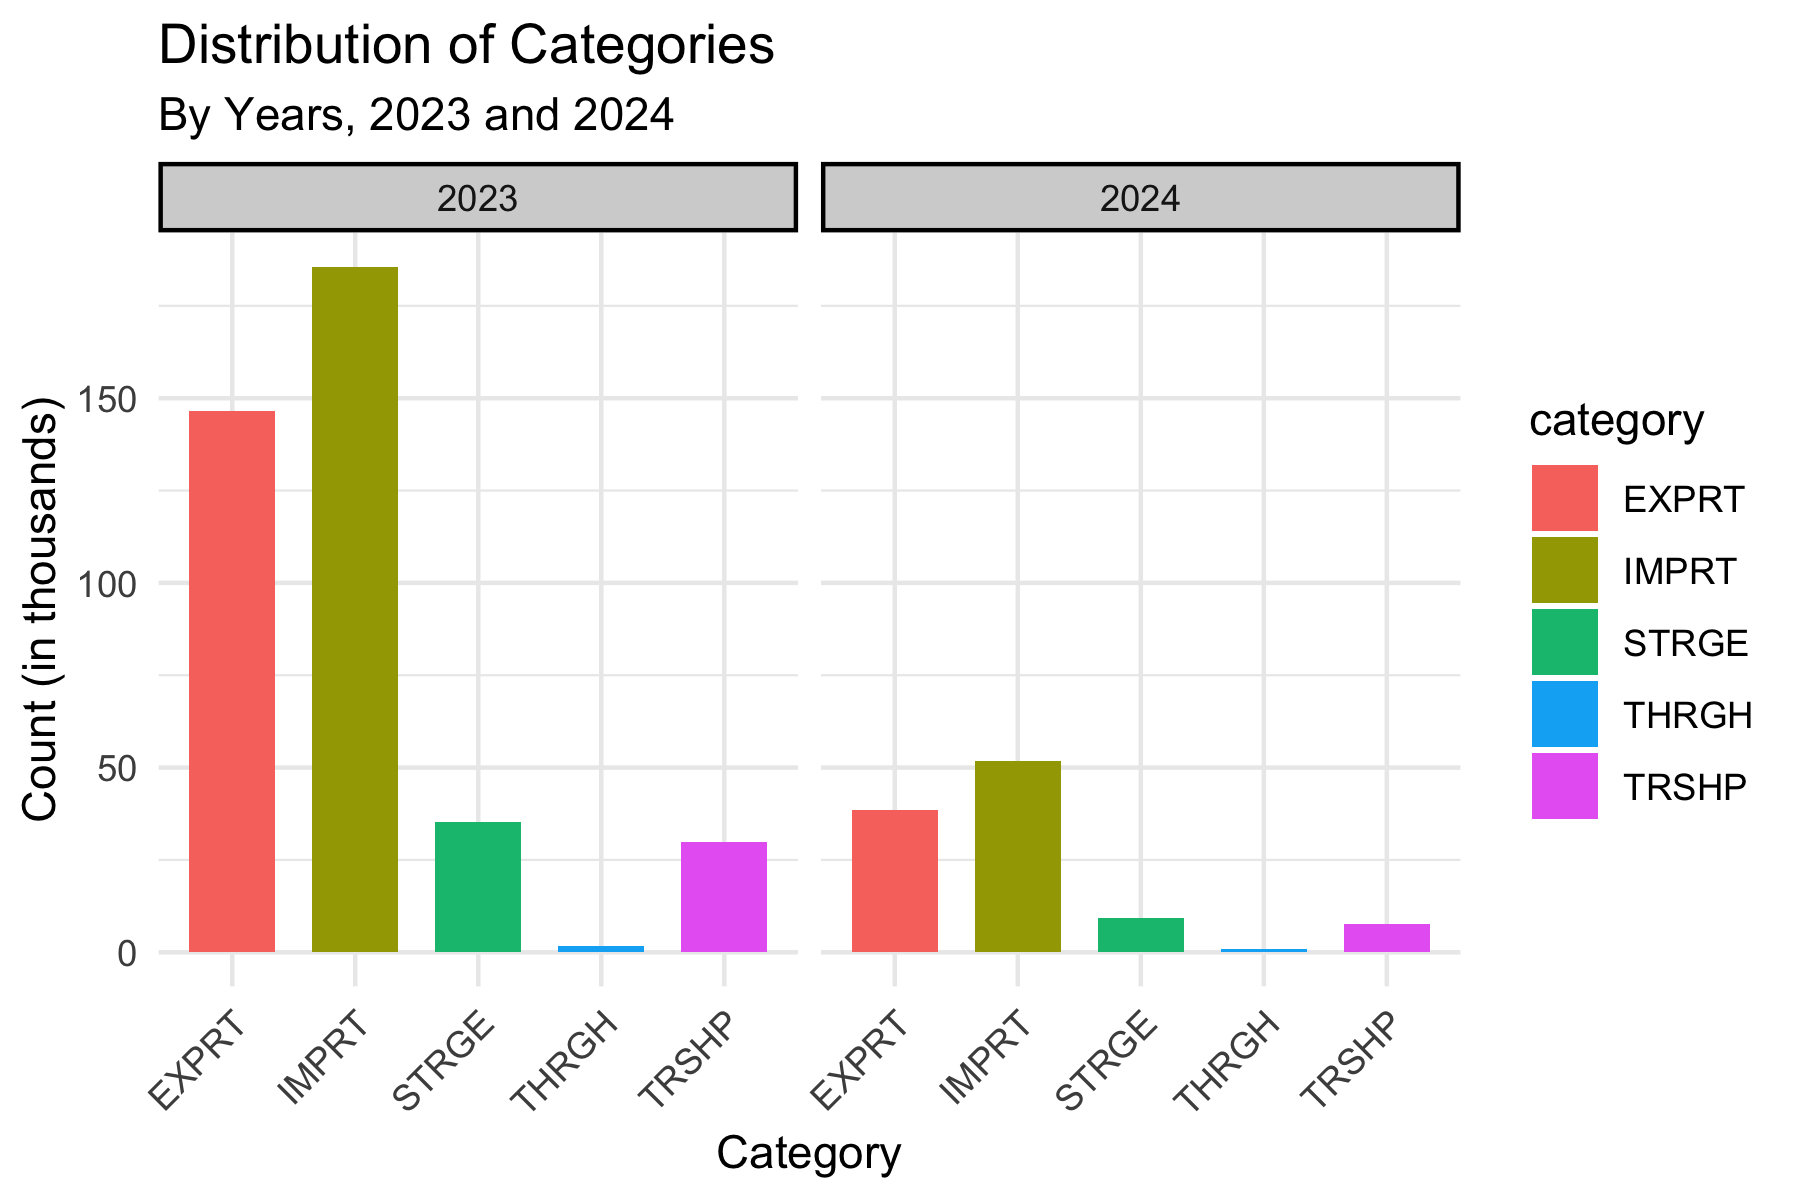
\includegraphics[width=0.5\textwidth]{images/du_five}
				\caption{Distribution of categories}
				\label{fig:category_distribution}
			\end{figure}
			\begin{figure}[ht]
				\centering
				\begin{minipage}{0.5\textwidth}
					\centering
					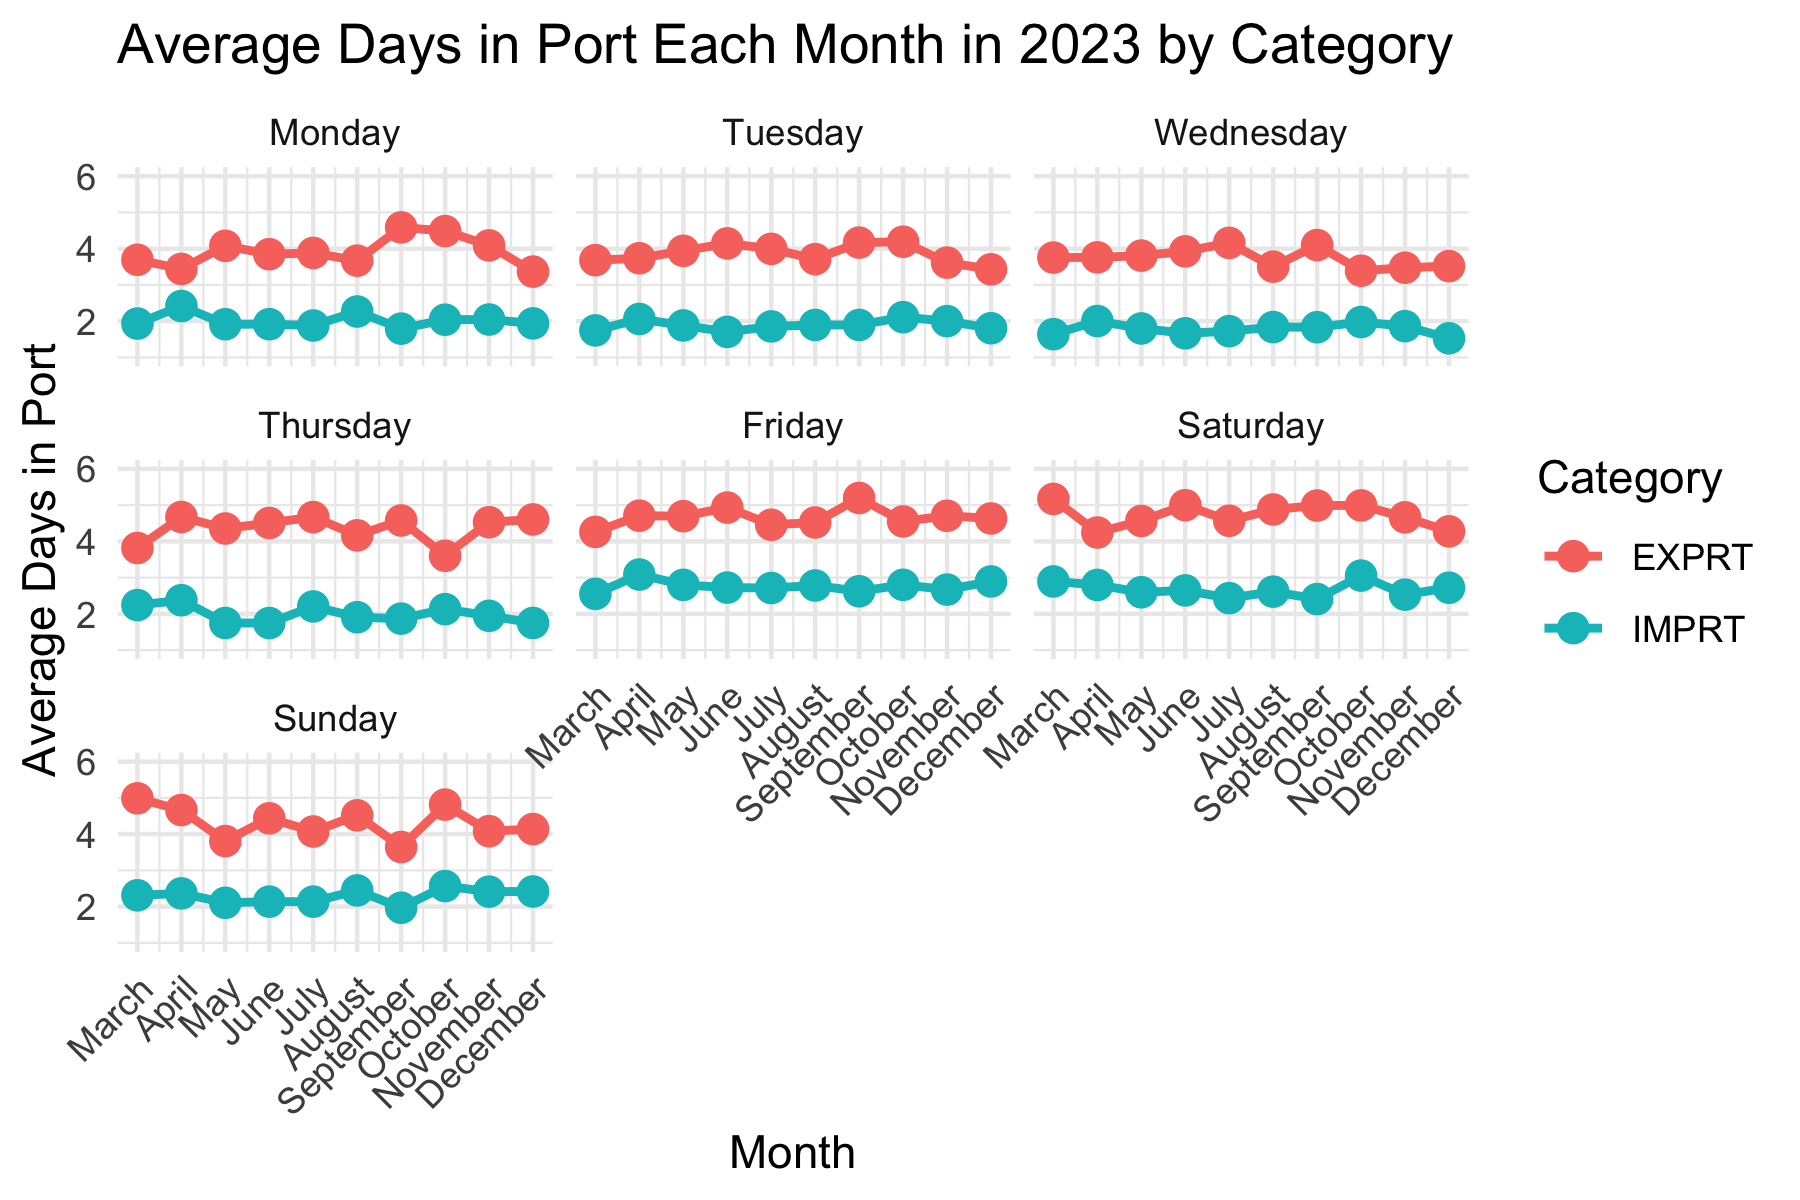
\includegraphics[width=\textwidth]{images/du_one}
					\caption{Month, day, and category}
					\label{fig:dwell_month_day_category}
				\end{minipage}%
				\hfill
				\begin{minipage}{0.5\textwidth}
					\centering
					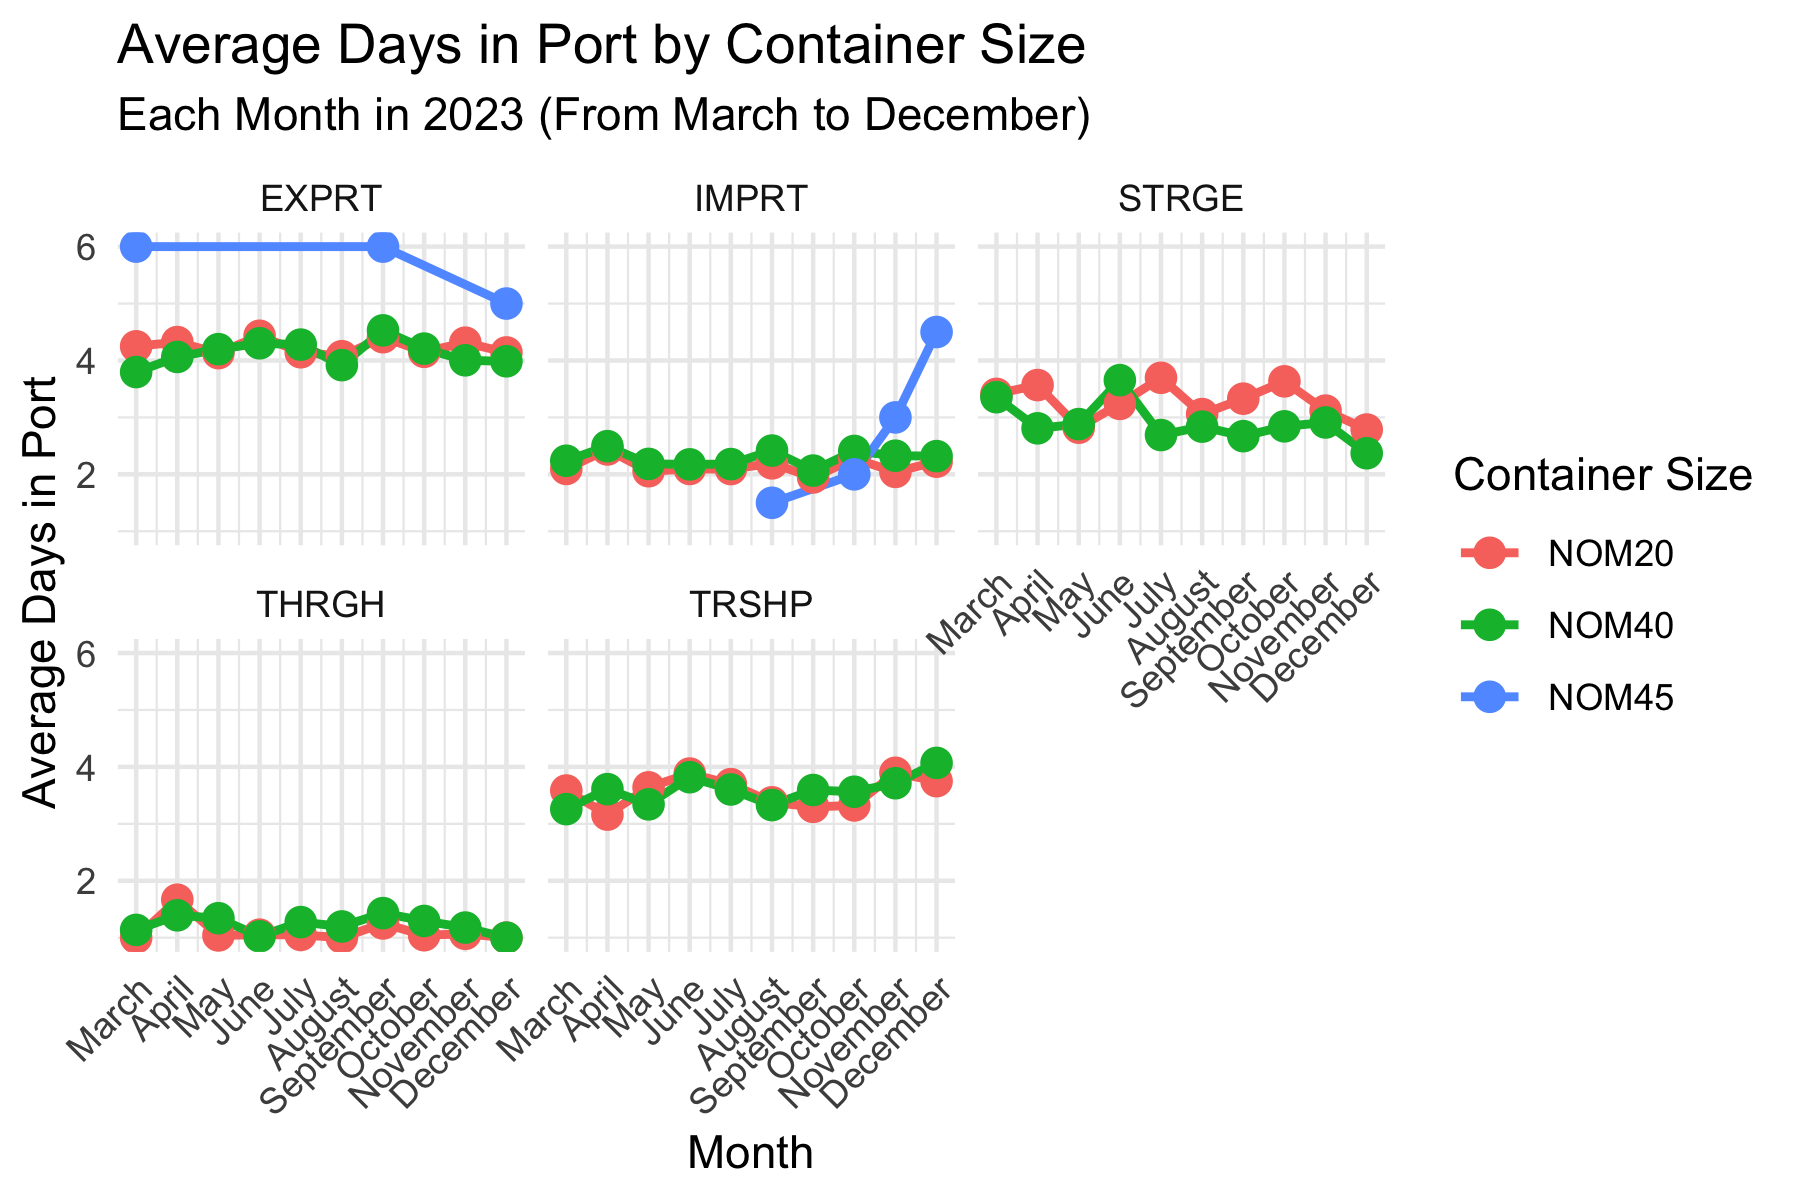
\includegraphics[width=\textwidth]{images/du_six}
					\caption{Month, category, and size}
					\label{fig:dwell_month_category_size}
				\end{minipage}
			\end{figure}
			Additionally, for categories, figure \ref{fig:dwell_month_day_category} shows patterns where export (
			EXPRT) containers consistently show higher dwell times (around 4 days) compared to import (IMPRT)
			containers (around 2 days) across all days of the week and the year. There is slight variation across
			weekdays, with Friday and Saturday showing marginally higher dwell times for both categories. Figure
			\ref{fig:category_distribution} shows the volume distribution across different operational categories,
			with IMPRT having the highest volume, followed by EXPRT in 2023 and 2024, though both show significant
			decreases in 2024. STRGE, THRGH, and TRSHP have notably lower volumes. figure
			\ref{fig:dwell_month_category_size} demonstrates how container size impacts dwell times across different
			operational categories - NOM45 containers show distinctly higher dwell times in EXPRT operations (around
			6 days) than NOM20 and NOM40 (around 4 days). In IMPRT operations, all container sizes show similar
			dwell times (around 2 days), while TRSHP shows more variability across container sizes. For predictive
			modeling, key features should include the day of the week (shown important in figure
			\ref{fig:dwell_month_day_category}), operational category (EXPRT/IMPRT/STRGE/THRGH/TRSHP as shown in
			Figure \ref{fig:category_distribution}), container size (NOM20/40/45 from figure
			\ref{fig:dwell_month_category_size}). The temporal patterns across days of the week (figure
			\ref{fig:dwell_month_day_category}) suggest that day-of-week and weekend/weekday indicators would be
			helpful to features.
			\\
			\\
			This analysis uncovered some patterns that influence how long containers stay in port. The timing of
			container arrivals matters significantly - there is a clear morning peak around 7-8 AM when containers tend
			to stay longer, and this varies across different days of the week and seasons. The category type plays a
			significant role: export containers consistently stay about twice as long as imports (4 days versus 2
			days), regardless of when they arrive. We have also seen empty containers generally stay longer than full
			ones, and larger containers (especially 45-footers) tend to need more time in port, particularly for
			exports. Given these findings, a predictive model should focus on three main aspects: when containers
			arrive (time of day, day of week, and season), what kind of operation they are part of (export, import,
			storage, etc.), and their physical characteristics (size and whether they are full or empty). Building
			models upon those found features could make it possible to develop solid predictors for how long
			containers will stay in port.